\documentclass[a4paper,11pt]{article}

\usepackage[T1]{polski}
\usepackage[utf8]{inputenc} 
\usepackage{graphicx}
\usepackage{float}
\usepackage{verbatim}
\hoffset=-3.0cm                 % Mniejszy lewy margines
\textwidth=18cm                 % szerzej
\evensidemargin=0pt

\voffset=-3cm                   % Mniejszy gorny margines
\textheight=27cm                % szerzej wzdluz

\usepackage{listings}
% Listingi
\lstdefinestyle{customc}{
	belowcaptionskip=1\baselineskip,
	breaklines=true,
	frame=L,
	xleftmargin=0pt,
	language=HTML,
	showstringspaces=false,
	basicstyle=\footnotesize\ttfamily,
	identifierstyle=\color{black}
}

\setlength{\parindent}{0pt}             % No paragraph indentation
\setlength{\parskip}{\medskipamount}    % Space between paragraphs
\raggedbottom   


\title{POLITECHNIKA WARSZAWSKA \\ WYDZIAŁ ELEKTRYCZNY \\}
\author{Michał Sut}
\date{\today}

\begin{document}
	\thispagestyle{empty}
	\maketitle
	\date{}
	\section{Treść zadania}
		Napisać program rozwiązujący problem komiwojażera (minimalizacja drogi pomiędzy n miastami bez powtórzeń) przy pomocy algorytmu genetycznego. Zastosować reprodukcję przy użyciu nieproporcjonalnej ruletki, operator krzyżowania CX oraz mutację równomierną.\\~\\
		Program powinien umożliwiać użycie różnych wielkości populacji, liczby iteracji, prawdopodobieństwa mutacji.
		\\~\\
		Program powinien zapewnić wizualizację wyników w postaci wykresów średniego, maksymalnego i minimalnego przystosowania (długości funkcji) dla kolejnych populacji oraz 2 map (o wymiarach 10x10 punktów), na których będą wyświetlane miasta oraz drogi najdłuższa i najkrótsza.
		\\~\\
		Pokazać działanie programu na danych testowych składających się z 10 miast, opisanych za pomocą współrzędnych na mapie o wymiarach 10x10 punktów.
		\\~\\
		Dane testowe: miasta:\\
		A(4,4), B(1,1), C(8,9), D(2,10), E(4,10), F(6,9), G(5,6), H(1,8), I(8,7), J(9,4)
	\section{Instrukcja działania programu}
		\subsection{Uruchomienie}
			Program został napisany w języku Python, z wykorzystaniem bibliotek zawartych w dystrybucji Anaconda. W związku z tym, należy uruchamiać program w tym środowisku. Można to zrobić poprzez zaimportowanie projektu do programu Visual Studio 2017, wybranie interpretera: Anaconda 4.2 i uruchomienie aplikacji. Plikiem startowym jest \texttt{ga.py}
		\subsection{Okno główne programu}
			\begin{figure}[H]
				\centering
				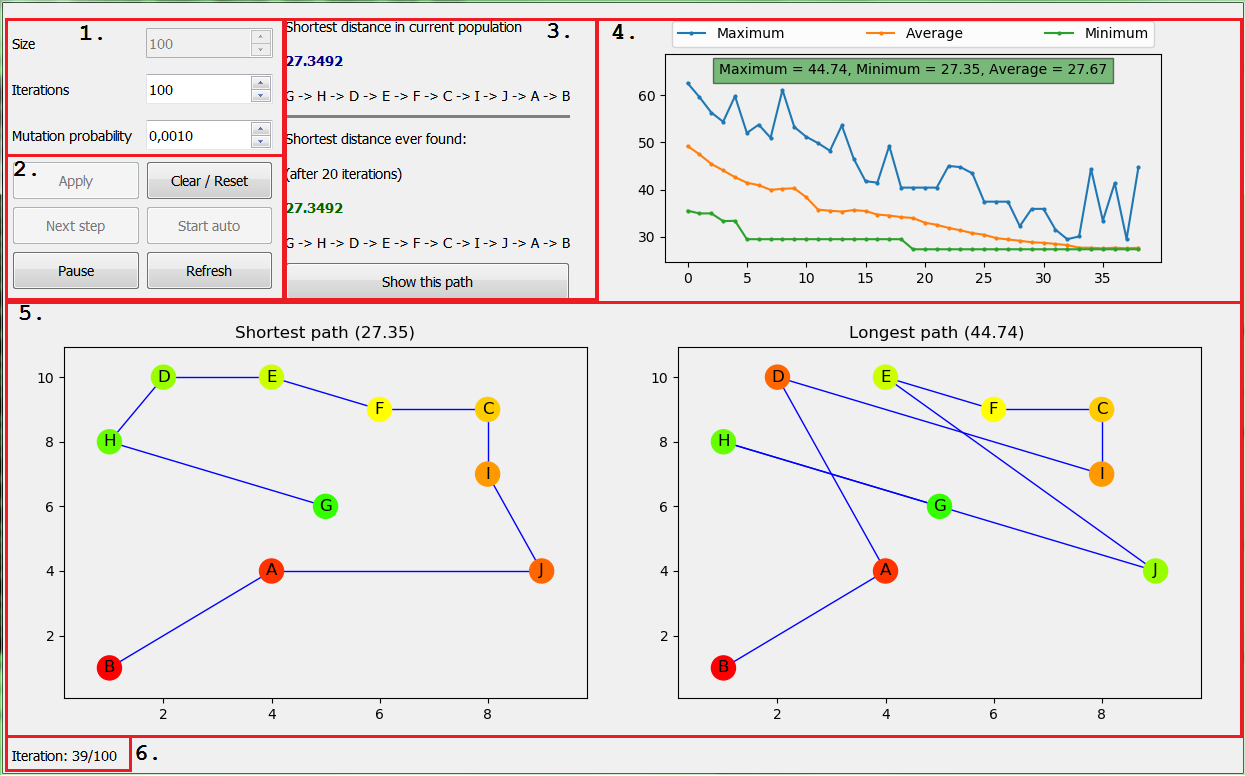
\includegraphics[scale=0.55]{main_window2.png}
			\end{figure}
		
		\subsection{Opis okna programu}
			\begin{enumerate}
				\item Parametry algorytmu
				\item Przyciski sterowania
				\item Informacje o najkrótszych znalezionych trasach
				\item Wykres wartości średnich, maksymalnych i minimalnych dla kolejnych generacji.
				\item Mapy z miastami i trasami: po lewej -- najkrótsza trasa, po prawej -- najdłuższa (Kolory oznaczają kolejność miast. Punkt początkowy jest najbardziej zielony, a punkt końcowy - najbardziej czerwony)
				\item Informacja o numerze aktualnej iteracji
			\end{enumerate}
		
		\subsection{Zmiana ustawień programu}
			Ustawienia programu znajdują się w pliku \texttt{settings.py}. Zmianą podlegają następujące elementy:
			\begin{enumerate}
				\item \textbf{CITIES} - Nazwy miast
				\item \textbf{POSITIONS} - Współrzędne miast
				\item \textbf{COLORS} - Kolory jakimi zaznaczane są kolejne miasta
			\end{enumerate}
	
		\subsection{Użycie}
			\subsubsection{Podstawowe operacje}
				\begin{enumerate}
					\item Ustawić parametry populacji
					\item Zainicjować populację klikając przycisk \framebox{ \texttt{Apply}}
					\item W tym momencie dostępne są trzy możliwości:
					\begin{enumerate}
						\item \framebox{Next Step} - Wykonanie tylko jednej generacji
						\item \framebox{Start Auto} - Wykonywanie kolejnych n generacji, gdzie n jest wybraną liczbą iteracji
						\item \framebox{Clear/Reset} - Wyczyszczenie populacji i zresetowanie programu
					\end{enumerate}
					\item Rozpoczęty proces automatycznych generacji można wstrzymać przyciskiem \framebox{Pause}
					\item Aby zobaczyć najkrótszą kiedykolwiek znalezioną trasę należy brać przycisk \framebox{Show this path}
				\end{enumerate}
			
		\subsection{Warunek stopu}
		Program zatrzymuje się po określonej liczbie iteracji, którą użytkownik określa w panelu ustawień parametrów algorytmu. Liczbę iteracji można zwiększać w trakcie działania programu.
		
	\section{Opis eksperymentów}
	Eksperymenty przeprowadzone były dla miast o następujących współrzędnych:  $$A(4,4), B(1,1), C(8,9), D(2,10), E(4,10), F(6,9), G(5,6), H(1,8), I(8,7), J(9,4)$$.
%	 Dokładność znalezionego rozwiązania obliczona jest poprzez obliczenie stosunku znalezionej wartości maksymalnej do wartości obliczonej analitycznie. W tym przypadku, maksimum funkcji wynosi $47$ i jest osiągane dla argumentu $x = 20$
	
		\subsection{Różna liczebność populacji}
			W celu przeprowadzenia tych eksperymentów, kilkukrotnie uruchomiony zostanie algorytm z następującymi parametrami: prawdopodobieństwo mutacji -- 0,001, liczba iteracji -- 200.
			\subsubsection{Populacja: 10 osobników}
				Wyniki prezentują się następująco:\\~\\
				\begin{tabular}{|c|c|c|c|c|}
					\hline 
					Lp & Min & Max & Mean & Best \\
					\hline
					1 & 31,63  & 34,72 & 33,48 & 31,63\\\hline
					2 & 35,36 & 35,36  &35,36 & 35,36 \\\hline
					3 & 35,99 & 35,99  & 35,99 &34,15 \\\hline
					4 & 31,08 & 31,08  & 31,08& 31,08 \\\hline
					5 & 31,96 & 31,96  & 31,96 & 31,96\\\hline
					&avg. min:&avg. max:&avg. mean:&avg. best:\\\hline
					& 33,20 & 33,82& 33,57 &32,84\\\hline
				\end{tabular} 
				
%				TU KONTYNUOWAC! !! !  ! ! 

			\subsubsection{Populacja: 50 osobników}
				Wyniki prezentują się następująco:\\~\\
				\begin{tabular}{|c|c|c|c|c|}
					\hline 
					Lp & Min & Max & Mean & Best \\
					\hline
					1 & 30.87 & 30.87 & 30.87 & 30.87 \\\hline
					2 & 28.28 & 37.84 & 28.47 & 28.28 \\\hline
					3 & 32.38 & 34.34 & 32.5 & 32.38 \\\hline
					4 & 31.76 & 31.76 & 31.76 & 31.76 \\\hline
					5 & 27.87 & 32.28 & 27.96 & 27.87 \\\hline
					&avg. min:&avg. max:&avg. mean:&avg. best:\\\hline
					& 30,14 & 33,42 & 30,31  & 30,11\\\hline
				\end{tabular} 
			\subsubsection{Populacja: 120 osobników}
				Wyniki prezentują się następująco:\\~\\
				\begin{tabular}{|c|c|c|c|c|}
					\hline 
					Lp & Min & Max & Mean & Best \\
					\hline
					1 & 24.59 & 24.59 & 24.59 & 24.59 \\\hline
					2 & 27.34 & 34.43 & 27.45 & 27.34 \\\hline
					3 & 24.59 & 28.66 & 24.62 & 24.59 \\\hline
					4 & 24.59 & 28.83 & 24.64 & 24.59 \\\hline
					5 & 24.59 & 24.59 & 24.59 & 24.59 \\\hline
					&avg. min:&avg. max:&avg. mean:&avg. best:\\\hline
					& 25.14 & 28.22 & 25.17 & 25.14 \\\hline
				\end{tabular} 
			\subsubsection{Populacja: 600 osobników}
				Wyniki prezentują się następująco:\\~\\
				\begin{tabular}{|c|c|c|c|c|}
					\hline 
					Lp & Min & Max & Mean & Best \\
					\hline
					1 & 27.35 & 44.16 & 27.5 & 27.35 \\\hline
					2 & 24.59 & 32.96 & 24.74 & 24.59 \\\hline
					3 & 24.59 & 41.4 & 24.75 & 24.59 \\\hline
					4 & 24.59 & 38.92 & 24.7 & 24.59 \\\hline
					5 & 24.59 & 41.4 & 24.69 & 24.59 \\\hline
					&avg. min:&avg. max:&avg. mean:&avg. best:\\\hline
					& 25.14 & 39.77 & 25.28 & 25.14 \\\hline
				\end{tabular} 
			\subsection{Różna liczba iteracji}
				Eksperymenty przeprowadzone będą dla populacji 250 osobników, z prawdopodobieństwem mutacji równym 0.001.
				\subsubsection{Liczba iteracji: 50}
					Wyniki prezentują się następująco:\\~\\
					\begin{tabular}{|c|c|c|c|c|}
						\hline 
						Lp & Min & Max & Mean & Best \\
						\hline
						1 & 27.35 & 40.03 & 28.09 & 27.35 \\\hline
						2 & 24.59 & 35.61 & 24.85 & 24.59 \\\hline
						3 & 29.59 & 36.61 & 29.81 & 29.59 \\\hline
						4 & 28.99 & 46.97 & 29.12 & 28.99 \\\hline
						5 & 24.59 & 40.6 & 24.76 & 24.59 \\\hline
						&avg. min:&avg. max:&avg. mean:&avg. best:\\\hline
						& 27.02 & 39.96 & 27.33 & 27.02 \\\hline
					\end{tabular} 
				\subsubsection{Liczba iteracji: 125}
					Wyniki prezentują się następująco:\\~\\
					\begin{tabular}{|c|c|c|c|c|}
						\hline 
						Lp & Min & Max & Mean & Best \\
						\hline
						1 & 24.59 & 40.65 & 24.79 & 24.59 \\\hline
						2 & 24.59 & 38.34 & 28.76 & 24.59 \\\hline
						3 & 27.93 & 29.35 & 27.93 & 27.93 \\\hline
						4 & 27.35 & 42.12 & 27.54 & 27.35 \\\hline
						5 & 24.59 & 37.26 & 26.25 & 24.59 \\\hline
						&avg. min:&avg. max:&avg. mean:&avg. best:\\\hline
						& 25.81 & 37.54 & 27.05 & 25.81 \\\hline
					\end{tabular} 
				\subsubsection{Liczba iteracji: 250}
					Wyniki prezentują się następująco:\\~\\
					\begin{tabular}{|c|c|c|c|c|}
						\hline 
						Lp & Min & Max & Mean & Best \\
						\hline
						1 & 24.59 & 41.61 & 24.84 & 24.59 \\\hline
						2 & 27.73 & 35.34 & 27.89 & 27.73 \\\hline
						3 & 27.35 & 40.4 & 27.48 & 27.35 \\\hline
						4 & 27.93 & 34.07 & 27.97 & 27.93 \\\hline
						5 & 27.35 & 44.37 & 27.49 & 27.35 \\\hline
						&avg. min:&avg. max:&avg. mean:&avg. best:\\\hline
						& 26.99 & 39.16 & 27.13 & 26.99 \\\hline
					\end{tabular} 
				\subsubsection{Liczba iteracji: 500}
					Wyniki prezentują się następująco:\\~\\
					\begin{tabular}{|c|c|c|c|c|}
						\hline 
						Lp & Min & Max & Mean & Best \\
						\hline
						1 & 29.03 & 39.89 & 29.17 & 29.03 \\\hline
						2 & 24.59 & 37.24 & 24.76 & 24.59 \\\hline
						3 & 29.76 & 43.78 & 29.9 & 29.76 \\\hline
						4 & 24.59 & 36.91 & 27.39 & 24.59 \\\hline
						5 & 29.03 & 35.8 & 29.1 & 29.03 \\\hline
						&avg. min:&avg. max:&avg. mean:&avg. best:\\\hline
						& 27.4 & 38.72 & 28.06 & 27.4 \\\hline
					\end{tabular} 
			\subsection{Różne prawdopodobieństwa mutacji}
				Eksperymenty przeprowadzone będą dla populacji 250 osobników. Liczba iteracji: 200
				\subsubsection{Mutacja: prawdopodobieństwo = 0,000}
					Wyniki prezentują się następująco:\\~\\
					\begin{tabular}{|c|c|c|c|c|}
						\hline 
						Lp & Min & Max & Mean & Best \\
						\hline
						1 & 30.11 & 30.11 & 30.11 & 30.11 \\\hline
						2 & 26.19 & 26.19 & 26.19 & 26.19 \\\hline
						3 & 28.88 & 28.88 & 28.88 & 28.88 \\\hline
						4 & 29.03 & 29.03 & 29.03 & 29.03 \\\hline
						5 & 26.37 & 26.37 & 26.37 & 26.37 \\\hline
						&avg. min:&avg. max:&avg. mean:&avg. best:\\\hline
						& 28.12 & 28.12 & 28.12 & 28.12 \\\hline
						
					\end{tabular} 
				\subsubsection{Mutacja: prawdopodobieństwo = 0,001}
					Wyniki prezentują się następująco:\\~\\
					\begin{tabular}{|c|c|c|c|c|}
						\hline 
						Lp & Min & Max & Mean & Best \\
						\hline
						1 & 24.59 & 34.09 & 24.72 & 24.59 \\\hline
						2 & 30.71 & 43.21 & 30.85 & 30.71 \\\hline
						3 & 27.35 & 40.81 & 27.71 & 27.35 \\\hline
						4 & 24.59 & 28.51 & 25.01 & 24.59 \\\hline
						5 & 27.35 & 40.18 & 27.58 & 27.35 \\\hline
						&avg. min:&avg. max:&avg. mean:&avg. best:\\\hline
						& 26.92 & 37.36 & 27.17 & 26.92 \\\hline
						
					\end{tabular} 
				\subsubsection{Mutacja: prawdopodobieństwo = 0,004}
					Wyniki prezentują się następująco:\\~\\
					\begin{tabular}{|c|c|c|c|c|}
						\hline 
						Lp & Min & Max & Mean & Best \\
						\hline
						1 & 24.59 & 42.02 & 25.39 & 24.59 \\\hline
						2 & 24.59 & 38.92 & 25.08 & 24.59 \\\hline
						3 & 24.59 & 39.19 & 25.28 & 24.59 \\\hline
						4 & 29.35 & 46.96 & 30.26 & 29.35 \\\hline
						5 & 24.59 & 42.56 & 25.29 & 24.59 \\\hline
						&avg. min:&avg. max:&avg. mean:&avg. best:\\\hline
						& 25.54 & 41.93 & 26.26 & 25.54 \\\hline
						
					\end{tabular} 
				\subsubsection{Mutacja: prawdopodobieństwo = 0,01}
					Wyniki prezentują się następująco:\\~\\
					\begin{tabular}{|c|c|c|c|c|}
						\hline 
						Lp & Min & Max & Mean & Best \\
						\hline
						1 & 29.24 & 49.74 & 30.65 & 29.24 \\\hline
						2 & 24.59 & 42.6 & 26.44 & 24.59 \\\hline
						3 & 29.03 & 53.71 & 31.79 & 29.03 \\\hline
						4 & 24.59 & 55.74 & 26.69 & 24.59 \\\hline
						5 & 24.59 & 45.19 & 26.35 & 24.59 \\\hline
						&avg. min:&avg. max:&avg. mean:&avg. best:\\\hline
						& 26.4 & 49.4 & 28.38 & 26.4 \\\hline
					\end{tabular}
%			\subsection{Podsumowanie eksperymentów}
%			\begin{tabular}{|c|c|c|}
%				\hline
%				Eksperyment & średnie maksimum & odchylenie stand. średniej maks. \\\hline
%				Populacja: 4  & 44,10 & 3,80\\\hline
%				Populacja: 10 &46,20 &1,10 \\\hline
%				Populacja: 50 & 46,66& 0,42\\\hline
%				Populacja: 100&46,77 &0,29\\\hline
%				Krzyżowanie: 1,00& 46,20 & 1,10 \\\hline
%				Krzyżowanie: 0,09& 45,03 & 0,88 \\\hline
%				Krzyżowanie: 0,05& 45,011 &2,65 \\\hline
%				Krzyżowanie: 0,00&  45,322 & 2,63\\\hline
%				Mutacja: 0,000& 41,3 & 3,49\\\hline
%				Mutacja: 0,001& 46,20 & 1,10\\\hline
%				Mutacja: 0,004& 46,58& 0,38 \\\hline
%			\end{tabular}
	\section{Wnioski}
		Przeprowadzone eksperymenty pokazują, że zmiana parametrów populacji wpływa na znajdowanie maksimum funkcji dopasowania danej populacji. 
		\subsection{Prawdopodobnie najlepsze rozwiązanie}
		Po przeprowadzeniu wszystkich eksperymentów, czyli uruchomieniu algorytmu 60 razy, można przypuszczać że najmniejsza z wartości, jaką podczas wszystkich prób udało się uzyskać, jest rozwiązaniem optymalnym lub przynajmniej jest zbliżona do wartości optymalnej. W tym przypadku, najmniejsza długość trasy, jaką udało się znaleźć, wynosiła: \textbf{24,5853}, a trasa ta to: \textbf{B -> A -> G -> D -> E -> F -> C -> I -> J}
		\subsection{Dokładność algorytmu}
		Algorytm nie zawsze znajduje najkrótszą możliwą drogę. W większości przypadków znajdowane były wartości bliskie oczekiwanej, czyli trasy, o długości zbliżonej do optymalnej. Na fakt znalezienia lub nie znalezienia optymalnego rozwiązania wpływają parametry populacji.
		\subsection{Wpływ wielkości populacji na wynik działania algorytmu}
		Przeprowadzone eksperymenty pokazują, że statystycznie lepsze wyniki uzyskiwane są dla większych populacji. Im większa populacja, tym większa szansa na znalezienie optymalnego rozwiązania. Przeprowadzone eksperymenty pokazały, że w większej populacji, wartość oszacowana jako najlepsza (w punkcie ,,4.1.'') była znajdowana najczęściej. Dodatkowo, im większa jest populacja, tym więcej iteracji potrzeba, aby populację zdominowało najlepsze rozwiązanie.
		\subsection{Wpływ liczby iteracji na wynik działania algorytmu} 
		Przeprowadzone badania pokazały, że im dłużej działa algorytm, tym lepsze wartości są znajdowane. Jest to szczególnie widocznie, przy małych populacjach, w których pośród początkowych wartości nie ma wartości optymalnych. W tym przypadku mutacje i krzyżowania muszą zajść więcej razy, aby udało się wygenerować coraz lepsze rozwiązania. \\
		Ponadto, z każdą kolejną iteracją etap reprodukcji zwiększa liczbę najlepszych rozwiązań w populacji, a zmniejsza liczbę tych najgorszych, co zwiększa szanse na znalezienie optymalnej wartości z każdą kolejną iteracją.
		\subsection{Wpływ prawdopodobieństwa mutacji na wynik działania algorytmu}
		Prawdopodobieństwo mutacji ma różny wpływ na działanie algorytmów w zależności od innego z parametrów: liczby osobników w populacji. Dla małych populacji, zwiększenie omawianego parametru powoduje, że generowane jest wiele nowych rozwiązań, wśród których mogą znajdować się osobniki bardziej przystosowane od obecnie istniejących w populacji. Jednakże, wraz ze wzrostem wielkości populacji, prawdopodobieństwo mutacji powinno się zmniejszać, aby uzyskiwać dobre wyniki. Dzieje się tak, ponieważ w większej populacji jest większa szansa na wystąpienie lepszych osobników. Mutacja może jednak wyeliminować te najlepsze wyniki, szczególnie w przypadku, gdy jest ich niewiele w populacji. \\
		Z drugiej strony, brak mutacji powoduje, że nowe rozwiązania znajdowane są znacznie rzadziej, ponieważ nowe rozwiązania powstają tylko w procesie krzyżowania. Dla zerowego prawdopodobieństwa mutacji, populacja zostaje szybko stosunkowo szybko zdominowana przez osobników o takim samym przystosowaniu.
	
\end{document}